\section{Thesis proposal}\label{sec:prelim}

\subsection{Project definition}
%I shall begin by restating many of the points covered throughout this literature review: The realisation of condensates was was first given in 1995, following prediction nearly 60 years previously. The behaviour of such systems saw much interest, with theoretical and experimental work seeing a significant rise since this date. One of the properties of condensates, the superfluid nature, received a large degree of attention, with many investigating the nature of quantised vorticity. Approaching the fast rotation limit allows these vortices to enter a crystalline lattice state, analogous to the Abrikosov lattice seen with type-II superconductors subjected to a static magnetic field. This mean-field quantum Hall regime remains predictable using the Gross--Pitaevskii equation, as it is still a weakly correlated state for a range of values beneath the fast-rotation limit. The use of optical lattices with condensates allows for the creation of strongly correlated states, giving a transition between Mott insulator and superfluid regimes by varying lattice intensity. Studies combining vortex lattices and optical lattices have shown transition from Abrikosov to pinned lattice state. Given the fluid superfluid nature of condensates it is possible to study chaos in the quantum regime. The kicked harmonic oscillator lends itself as an ideal model to attempt an understanding of chaos in quantum systems, and has been demonstrated as such.
As part of my PhD I intend to investigate the dynamical behaviour of Bose--Einstein condensates within the fast-rotation limit. With the rotation frequency approaching the trapping frequency of the condensate, the appearance of an Abrikosov (triangular) lattice of vortices in the condensate is expected. This is similar to the type of behaviour observed in type-II superconductors subjected to an applied magnetic field \cite{QM:Abrikosov_jpcs_1957}. With the condensate ground-state having an Abrikosov lattice of vortices, the goal will be to investigate quantum dynamical behaviour in this mean-field quantum Hall regime, with an investigation into chaotic dynamics. This will be carried out by treating the system as a delta-kicked quantum oscillator, where a periodically pulsed optical lattice, whose structure is matched to that of the vortex lattice, is doing the kicking. The plan is to treat the vortex as an effective particle through which the (potentially chaotic) dynamical behaviour may be observed. The Hamiltonian of this system can be mapped to that of the delta-kicked harmonic oscillator Hamiltonian, and will allow for a means to describe the resulting dynamics using an analytical  approach.
%The delta kicking shall be from an intense Gaussian laser field, applied to the vortex position at timescales shorter than the condensate dynamics. However, dealing with a single vortex and single narrow laser is possible, more experimentally realisable, and useful information may be obtained from the use of a large collection of vortices, such as the Abrikosov lattice. The subjecting laser field shall thus be given as that of an optical lattice, with structure matching that of the vortex lattice.

Due to the complex nature of this proposed system, a significant degree of computation will be required. Following on from the methods given in Section \ref{sec:numerics}, one way to perform the large computations required are through use of graphics processing units (GPU). I have previously worked on developing an application for the numerical solution of a fully three-dimensional Schr\"{o}dinger equation in waveguides using GPUs \cite{AO:Morgan_pra_2013}, and I have used this as the basis for the study proposed. I have further modified the developed code to deal with the non-linearity arising from the Gross--Pitaesvkii equation \eqref{eqn:gpe_rotation}, and to account for angular momentum. The resulting code was published under an open-source LGPLv2 license, and named ``GPUE'' \cite{NUM:gpue}. Generalisation of this code will allow more complex quantum systems to be examined, and so far has been shown to achieve results in substantially less time than competing implementations.

%For a thorough understanding of the numerically obtained results, more complex analytics will be considered and applied. For this the Wigner quasi-probability function will be calculated, to allow observation of the phase-space dynamics of the system. I will also apply Floquet theory to this periodic system, which will allow the derivation of analytical results in certain limits.
%Once the code to determine the ground-state under large rotation is developed, the preparation of a vortex lattice with any specified number of vortices is expected to be numerically possible. Such a system may then be pulsed via briefly applied external potentials. Considering the use of a triangular optical lattice, wherein the lattice spacing is equivalent to the inter-vortex spacing of the condensate, a 1:1 mapping of the optical lattice to the vortex lattice can be achieved within a certain condensate radius. The goal of my project is to create a system in which behaviour akin to that of the delta-kicked quantum oscillator can be observed and to study the potentially chaotic dynamics. Treating the vortex as an effective particle, and the optical lattice potential as a delta perturbation in time, it may be possible to observe signatures of chaos for topological excitations. %Quantification of quantum chaos in experimentally realisable systems, such as superfluid Helium, is a challenging feat \cite{CT:Kobayashi_pra_2007}. The use of dilute condensates instead of superfluid Helium offers much greater ease in observing phase and density, and as such these systems may offer more insight into, and showcasing of the dynamics that can be expected to occur.

To effectively study this system, it will be necessary to obtain a thorough understanding of both classical and quantum chaos for
Hamiltonian systems. Properties of the system will be analysed, with phase-space methods, such as calculating the Wigner function, which will provide information about the system dynamics \cite{CT:Gardiner_pra_2000}. It will be necessary to calculate the Wigner function for each variation of the condensate system parameters, and further indepth studies using Floquet analysis will be necessary for effective characterization of the observed behaviours \cite{CT:chu_physrep_2004,CT:McCaw_thesis_2005,CT:Gardiner_thesis_2000,CT:Kells_pre_2004}.

\subsection{Overall aims}
For successful completion of this project the following goals are outlined.
\begin{itemize}
	\item Generate a large, stable vortex lattice using a Bose--Einstein condensate within the MFQH regime.\vspace{-1em}
	\item Generate dynamical simulations of BECs using a periodically pulsed optical lattice matched to vortex lattice.\vspace{-1em}
	\item Track the motion of individual vortices in position space, and characterise dynamical behaviour observed.\vspace{-1em}
	\item Analyse the behaviour of the system in phase-space using the Wigner function of the resulting dynamics.\vspace{-1em}
	\item Apply Floquet theory to the system, and infer information about the observed behaviour from the results.
\end{itemize}
Experiments to observe chaotic behaviour in the quantum regime are rare, and the realisation of this type of system should allow for the first of its kind to observe chaos in a system of well-ordered topological excitations. Given recent experimental progress in the area of trapping, cooling, rotating and controlling Bose--Einstein condensates, the proposed system should be realisable with currently available experimental techniques.
The required techniques for theoretically performing this body of work will be described below.

\subsection{Methods and techniques}
\subsubsection{Creating a vortex with phase imprinting}
As a precursor to this proposal, I have performed preliminary work during my time in the Busch unit to investigate the behaviour of condensates with differing numbers of
vortices, and subjected to a short external pulse. Initially, the behaviour of a condensate with a low number of vortices (0,1,2) was examined.
Numerical integration of the two dimensional Gross--Pitaevskii equation in imaginary time in the co-rotating frame allowed for the
determination of the ground-state in the absence of the perturbation. A predefined winding number, corresponding to the number of vortices required, was applied by multiplication of an appropriate phase with an initial Gaussian guess for the wavefunction guess, and evolved in imaginary time. After that, the resulting numerical ground-state solution was perturbed by kicking it with an additional Gaussian phase pattern, representing a laser pulse (kick), and he system was evolved in real time. A Gaussian phase is
known to give rise to breathing modes in the condensate \cite{BEC:Kimura_pra_2002}, as the velocity of the condensate atoms is given by the
gradient of its phase. With a kick of large amplitude, the atoms with sufficiently steep phase gradient will move at a greater velocity than those at the
edges or the centre of the Gaussian pulse. As a result, the faster moving atoms will overtake those in the slower moving regions, and due to the
coherent nature of the condensate, matter-wave intereference fringes were observed. From this observation, it is clear that the condensate
under these conditions behaves as an interferometer. With the presence of more than a single Gaussian pulse more complex interference
patterns can develop and any inhomogeneities in the trapping potential will give rise to a non-symmetric fringe pattern, which may in turn be used to determine the quality of the trap, or the topology of nearby structures. Example results are shown in Fig. \ref{FIG:bec_fringe}.
\begin{figure}[tb]
\begin{center}
	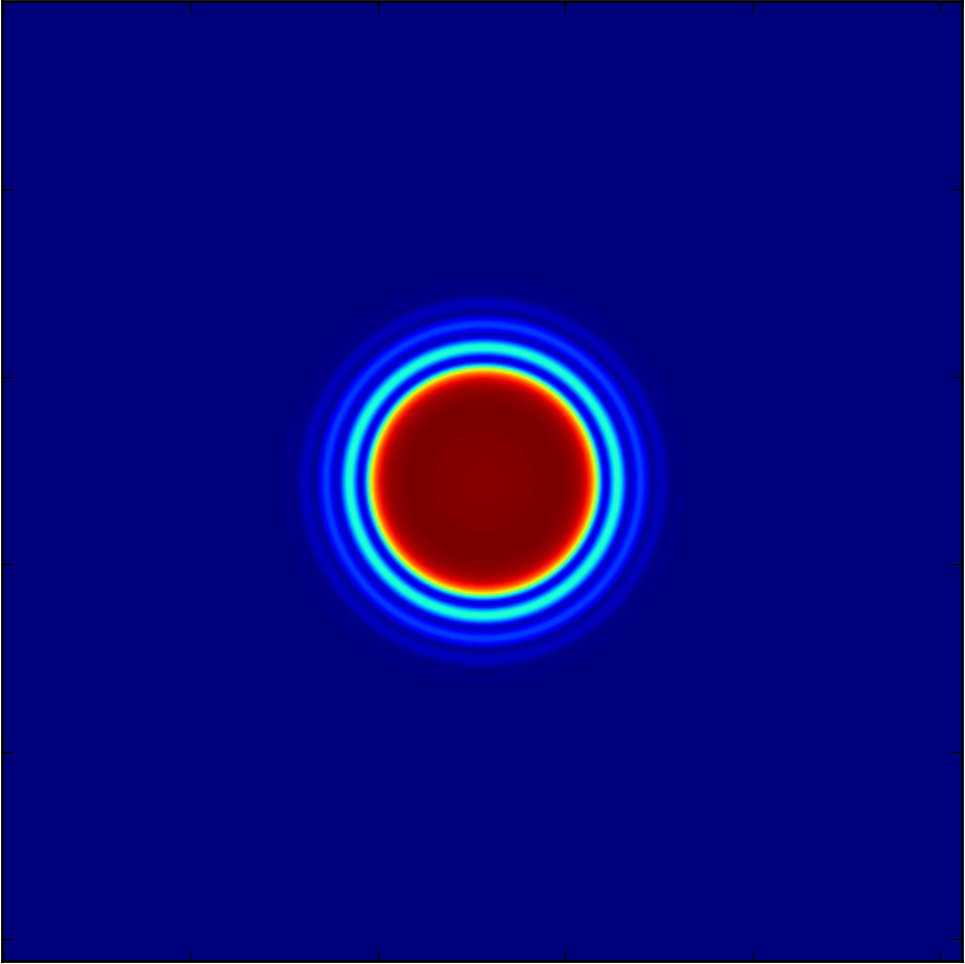
\includegraphics[trim=10cm 10cm 10cm 10cm, clip, scale=0.25,width=3cm]{ch1_litrev/symmetric_guassian_no_vortex_expansion.png}\vspace{0.1em}
	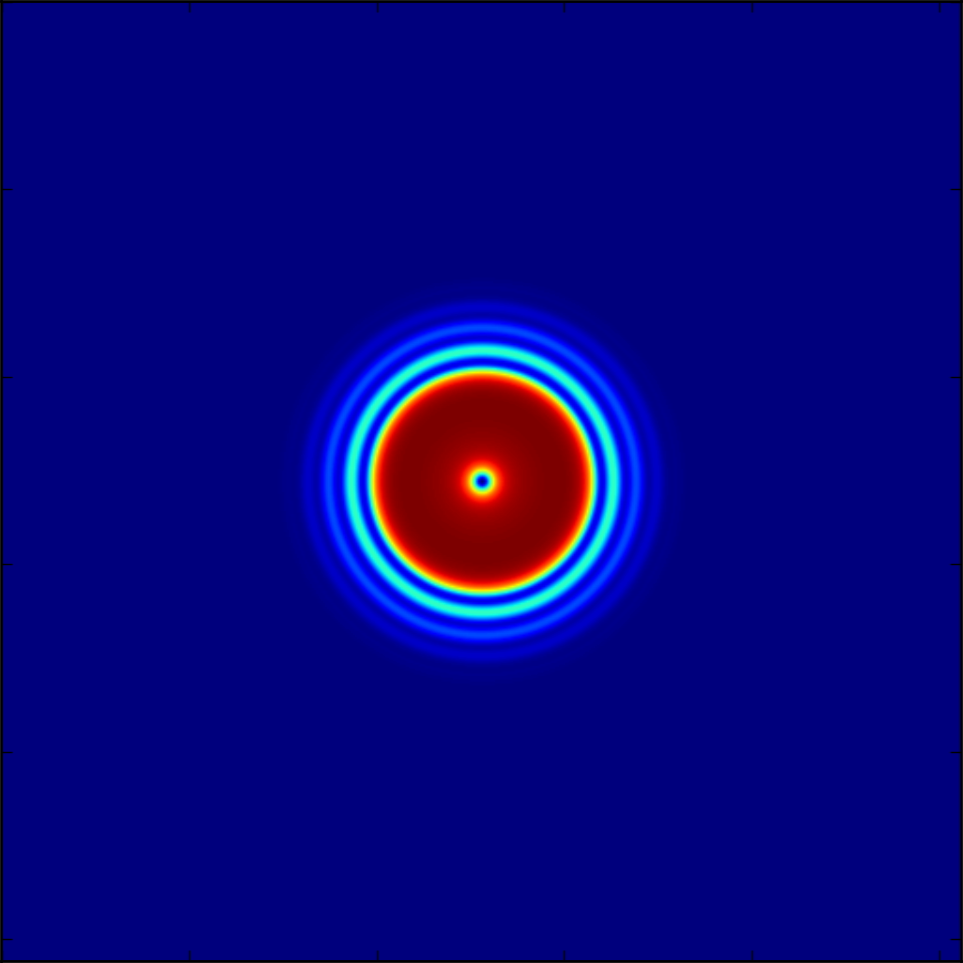
\includegraphics[trim=10cm 10cm 10cm 10cm, clip, scale=0.25,width=3cm]{ch1_litrev/symmetric_gaussian_centre_1vortex_fringe_1stexpansion.png}
	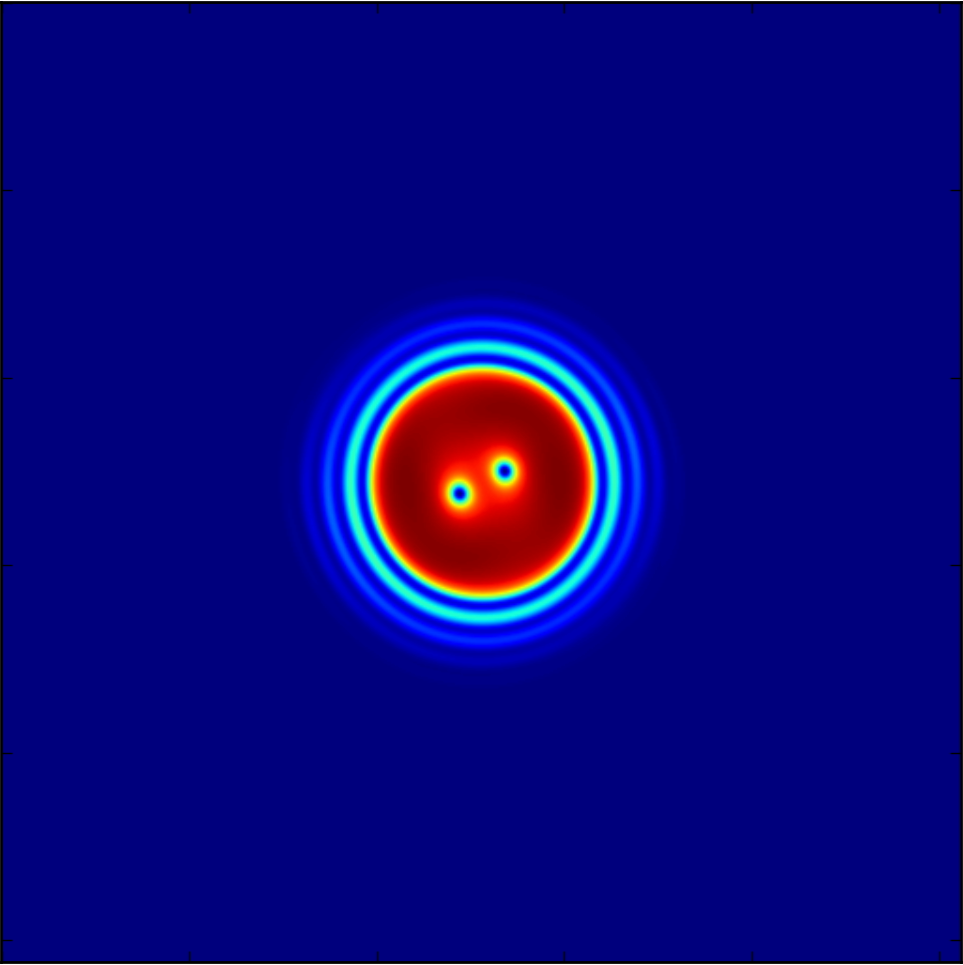
\includegraphics[trim=10cm 10cm 10cm 10cm, clip, scale=0.25,width=3cm]{ch1_litrev/rotating_2vortex_gaussian_centre_1stexpansion.png}
	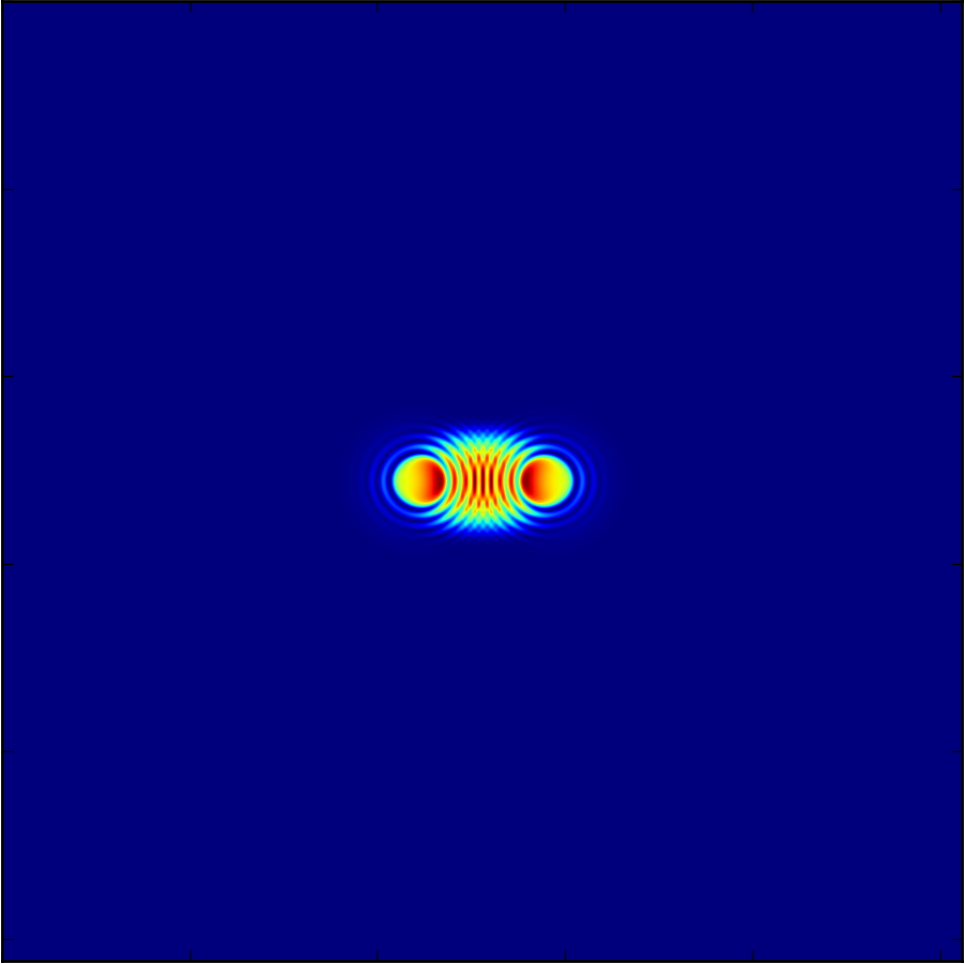
\includegraphics[trim=12cm 12cm 12cm 12cm, clip, scale=0.25,width=3cm,height=3cm]{ch1_litrev/assymetric_0vortex_gaussian_left_right_higher_power.png}


	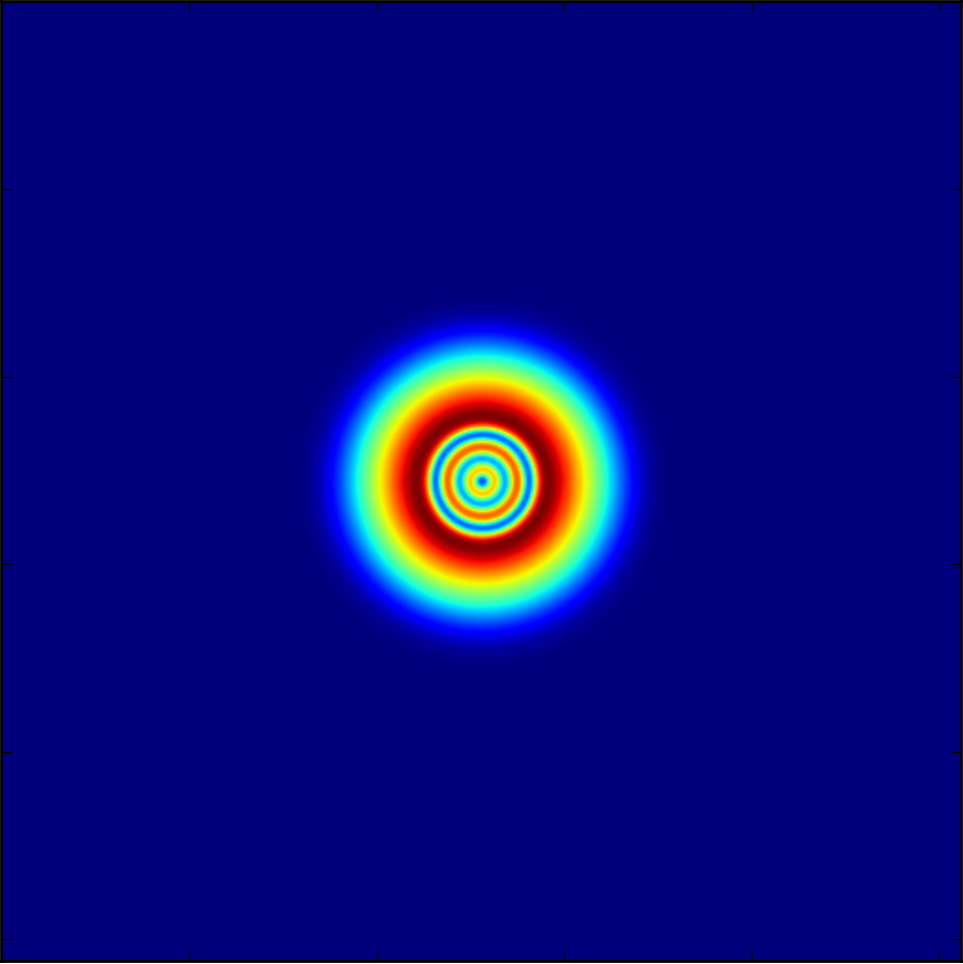
\includegraphics[trim=10.1cm 10cm 10.1cm 10cm, clip, scale=0.25,width=3cm]{ch1_litrev/symmetric_guassian_no_vortex_contraction.png}
	\includegraphics[trim=10.1cm 10cm 10.1cm 10cm, clip, scale=0.25,width=3cm]{ch1_litrev/symmetric_gaussian_centre_1vortex_fringe_1stcontraction.png}
	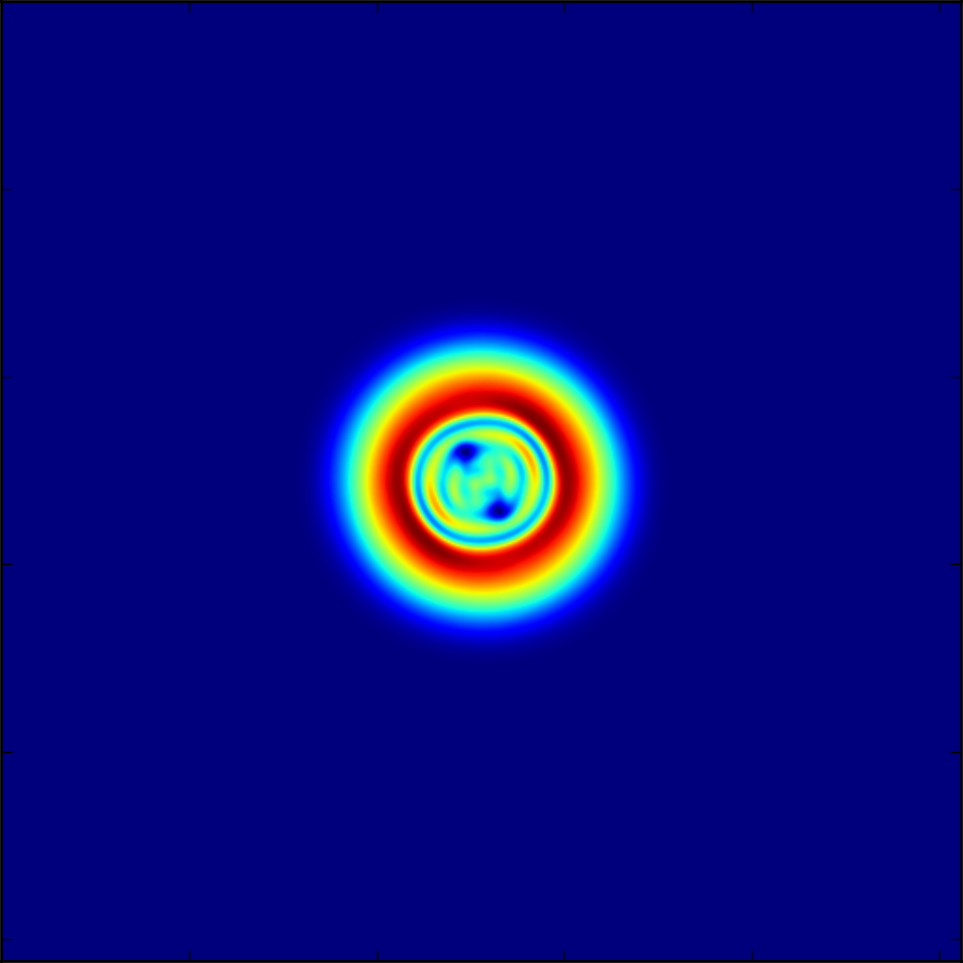
\includegraphics[trim=10.1cm 10cm 10.1cm 10cm, clip, scale=0.25,width=3cm]{ch1_litrev/rotating_2vortex_gaussian_centre_1stcontraction.png}
	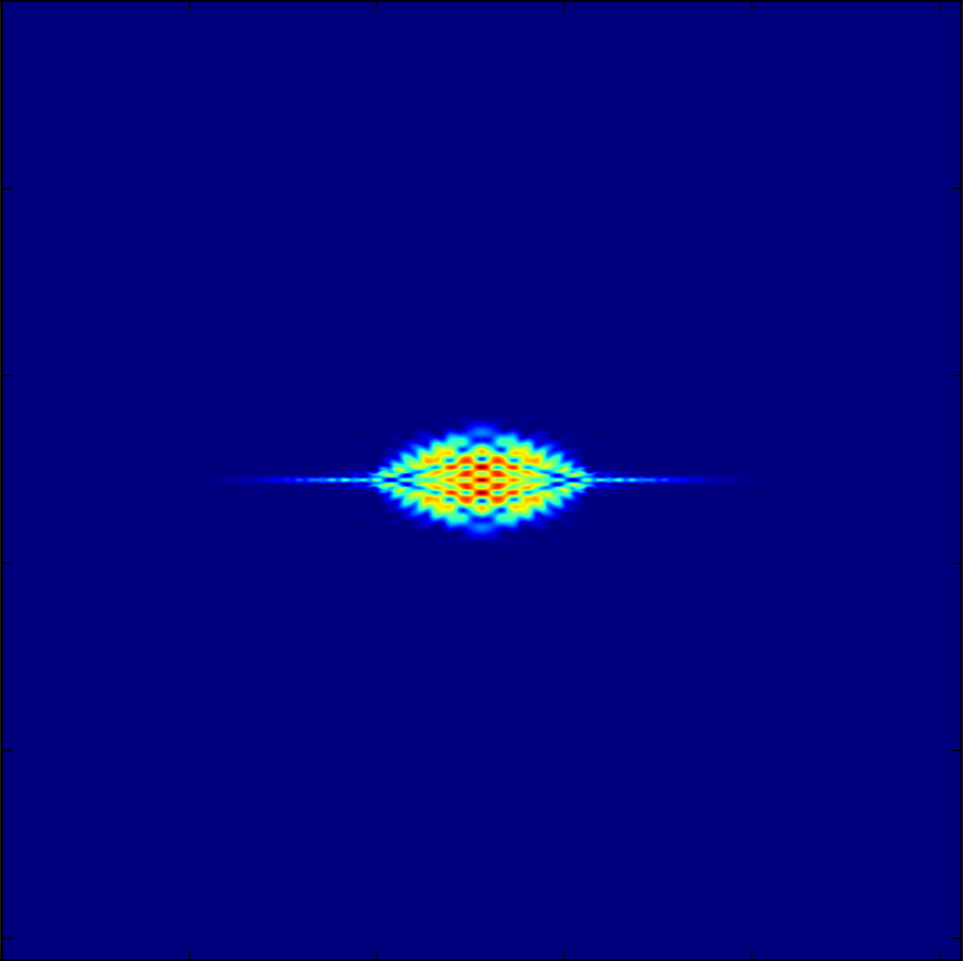
\includegraphics[trim=12cm 12cm 12cm 12cm, clip, scale=0.25,width=3cm,height=3cm]{ch1_litrev/asymetric_novortex_dual_gaussian.png}
	%\includegraphics[trim=10.1cm 10cm 10.1cm 10cm, clip, scale=0.25,width=3cm]{images/symmetric_gaussian_centre_1vortex_fringe_1stcontraction.png}
\end{center}\vspace*{0pt}\caption{Sample results of BECs with varying number of vortices subjected to different phase imprinted patterns. Images are paired top and bottom, at different stages of evolution. From left to right the examined systems are: (i) harmonically trapped condensate with no vortex plus a Gaussian phase in centre; (ii) harmonically trapped condensate with a single vortex plus a Gaussian phase in centre; (iii) harmonically trapped condensate with two vortices plus a Gaussian phase in centre; (iv) anharmonically trapped condensate with no vortex plus two Gaussian phase patterns on opposite sides of condensate\vspace*{-10pt}}\label{FIG:bec_fringe}
\end{figure}

\subsubsection{Creating a vortex lattice}
At low values of the rotation ($0 \leq \Omega \leq 0.49\omega_{\perp}$) the condensate can support a small number of vortices, which when evolved
in imaginary time will form a uniform structure. Increasing the rotation frequency further ($0.5\omega_{\perp} \leq \Omega \leq 0.89\omega_{\perp}$) allows the condensate to support a much larger number of vortices, which can arrange themselves into a lattice pattern. At values approaching the limiting frequency the vortices should order into a large Abrikosov lattice pattern, similar to what
is observed in type-II superconductors. Starting with a large winding number for the phase imprint pattern, the resulting initial guess is evolved in imaginary time, and values approaching the fast rotation limit were chosen. Figure \ref{fig:close_to_abrikosov} shows an example of the condensate under fast rotation, assuming an initial winding of the order 100.
 \begin{figure}[tb]
 \centering
 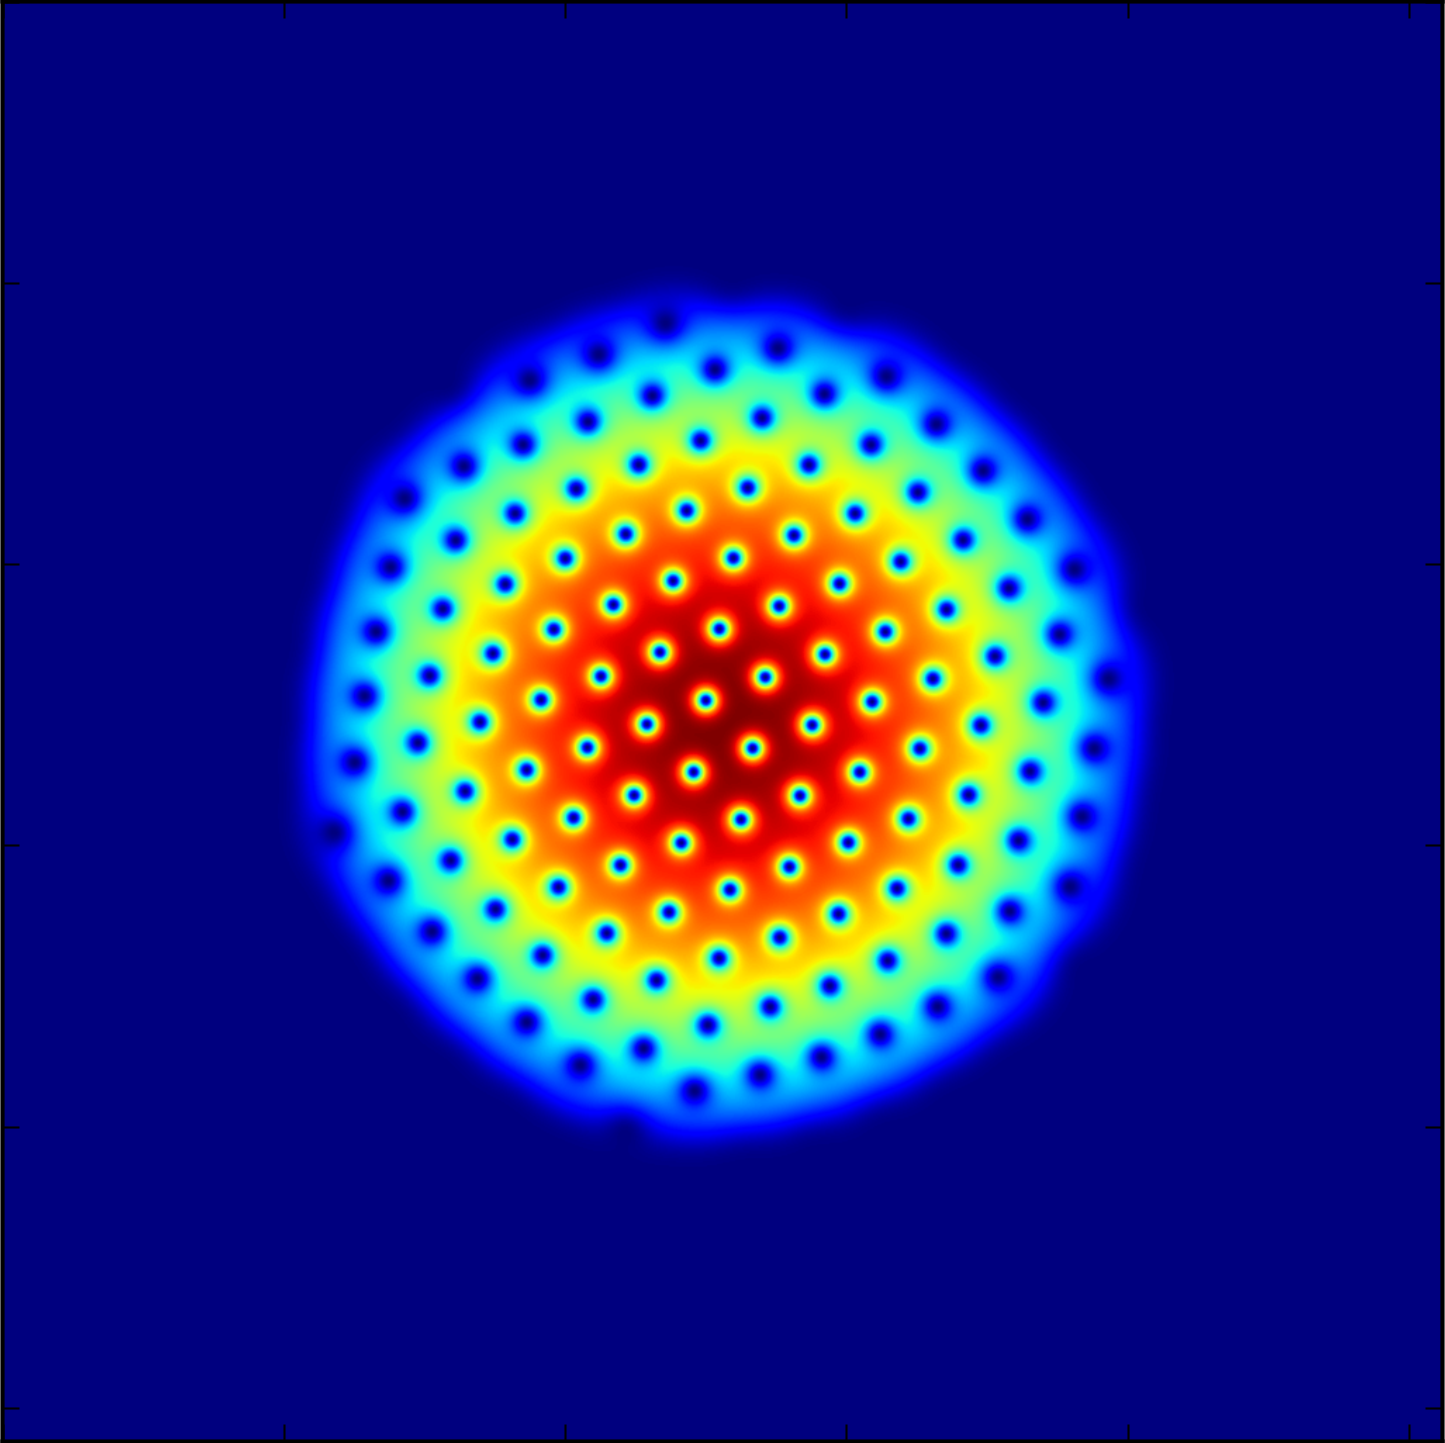
\includegraphics[scale=0.085]{ch1_litrev/wfc_19900000.png}
  \includegraphics[scale=0.085]{ch1_litrev/phi_19900000.png}
  \caption{Images show the ground-state of a condensate rotating at a frequency of $\Omega=0.9\omega_{\perp}$. Even though the Abrikosov lattice is clearly visible, a number of imperfections can be seen in the vortex alignment. Left image shows density, right image shows the phase.}
  %, evaluated at a timestep of $2\times 10^{-6}$ over a grid of $2^{10}\times 2^{10}$
  \label{fig:close_to_abrikosov}
 \end{figure}
To simulate this type of system careful consideration of the angular momentum term in the Hamiltonian must be taken. Initial results have been obtained through use of the GPUE codes that I have developed. However,  the implemented algorithm fails to botain a stable vortex lattice at large rotational frequencies, and so will require an alternative treatment of the system to generate the required state.

\subsubsection{Triangular optical lattice pattern}
For the optical lattice potential, three retroreflected laser fields are considered, giving rise to plane-waves oriented at 0, $\pi/3$ and $2\pi/3$. The resulting fields are defined as
\begin{equation}\label{eqn:lattice_potential_tri}
V_{opt} = V_0\left[\cos^2\left(k\frac{x-\sqrt{3}y}{2} \right) + \cos^2\left(k\frac{x+\sqrt{3}y}{2} \right) +\cos^2\left(ky\right)\right],
\end{equation}
where $V_0$ is the amplitude of the optical lattice, and $k$ is the wavevector, given by $k=2\pi/\lambda$. A sample resulting optical lattice potential is shown in Fig. \ref{fig:optical_lattice}. The optical wavelength and position can be precisely controlled, even though it is an experimentally challenging task. Given the fine control over condensate parameters, matching the optical lattice to the vortex lattice structure is expected to be experimentally realisable, albeit with cutting edge techniques \cite{Vtx:Tung_prl_2006}.
\begin{figure}
\centering
	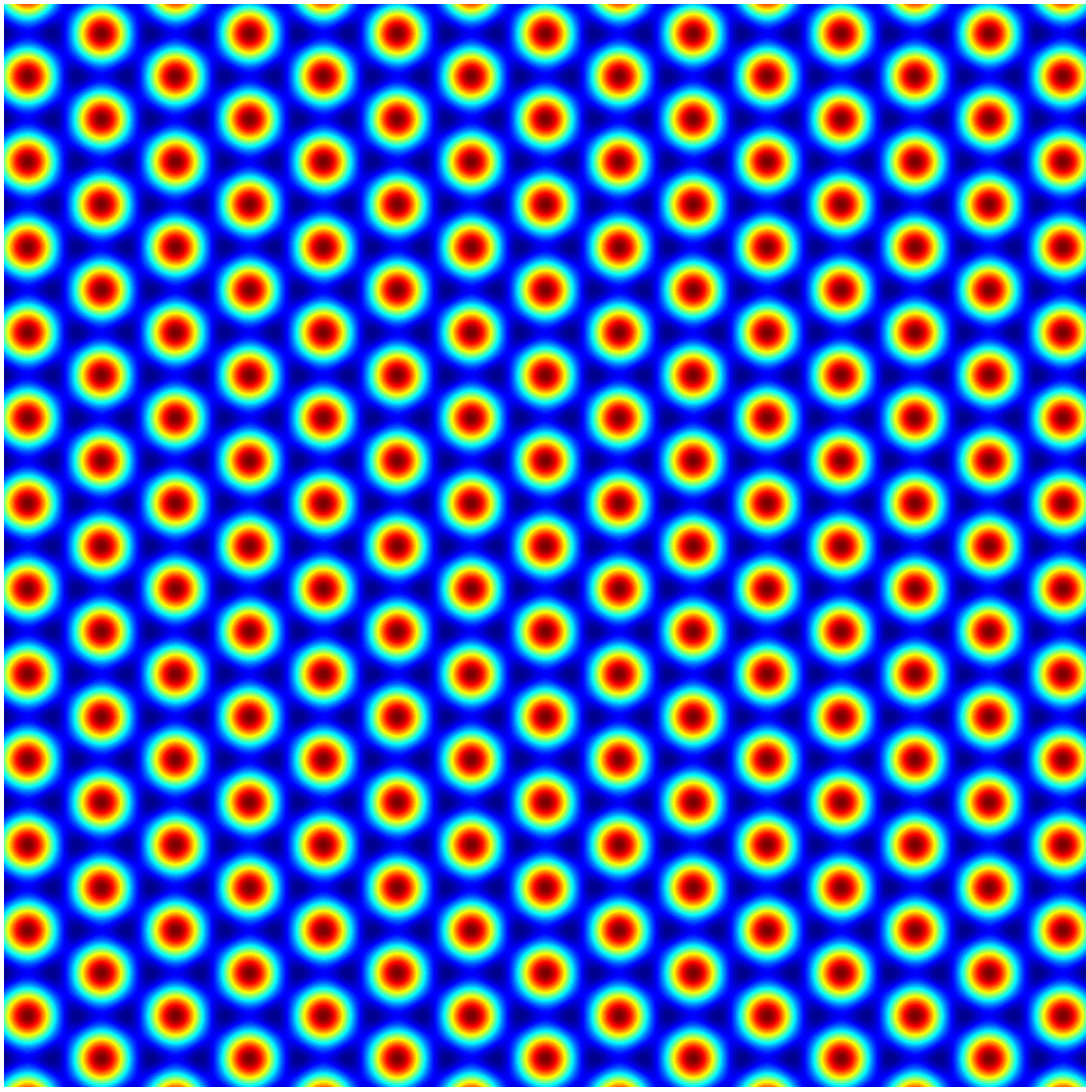
\includegraphics[scale=0.2]{ch1_litrev/opt_latt_g.png}
	\caption{The above image shows a triangular optical lattice potential pattern. This pattern will be adjusted to match the Abrikosov lattice pattern of the condensate in the fast-rotation limit.}\label{fig:optical_lattice}
\end{figure}
To use this optical lattice to generate the expected dynamics in the simulation it will be applied during the real-time evolution. This can be allowed by summing with the trapping potential for an instantaneous pulse of timescale equal to the time-step, or can be applied directly to the condensate phase.

\subsubsection{Delta kicked harmonic oscillator}
Using the Abrikosov lattice pattern with the triangular optical lattice potential we can map this system to the delta-kicked harmonic oscillator, presented in Section \ref{sec:chaos}. In the fast rotation limit, with an Abrikosov lattice pattern of vortices, the lattice undergoes a solid-body rotation. Given that the Abrikosov lattice is a triangular lattice pattern, the system has six-fold rotational symmetry, corresponding with a rotation of $\pi/3$ radians. Thus, a kick applied after a rotation through multiples of this angle will provide a periodic pulsing. The time to rotate through this angle will give the required period, $\tau$, of the system. The amplitude of the optical lattice pattern
will yield the kicking strength, $K$. It is expected that after a yet undetermined number of initial kicks the vortices will start interacting and move from an Abrikosov geometry. After this, all vortices will feel subsequent kicks with a strength dependent upon distance from the maxima and minima of the optical lattice, and should yield some chaotic dynamics. The chaotic dynamics of the system will be investigated by observing the motion of the vortices after a variable total number of kicks, choice of kicking period, lattice size, kicking strength, and a range of interaction strengths for the condensate. Further dynamical behaviour may be determined by calculating the Wigner distribution of the resulting wave-function, and also by analytical analysis using a Floquet theory approach.

\subsection{Significance of proposed work}
The extension between classical and quantum systems remains to be understood. At the classical--quantum limit, the observation of chaos offers a way to gain some insight into processes that may occur. Currently there have been no studies of quantum chaos in systems of topological excitations. Undertaken this project would be the first into investigating such behaviour, and as a result many interesting new physics may be observed. Characterisation of the chaotic behaviour observed in this type of system also will allow for comparative works between the classical and quantum cases. This is a newly developing area of investigation, and the use of condensate use investigating chaotic behaviour has seen few experimental realisations to date. The outlined set-up would allow for a highly controllable system to be subjected to a periodic perturbation relatively easily, mapping it well to the kicked harmonic oscillator. The resulting numerical routines developed should allow for a variety of physical phenomena to be investigated in much shorter timescales compared to currently available methods.

An extension of the work proposed in the project can go in many related directions. One possibility would be to study the transition from the mean-field regime to the strongly correlated (e.g. Mott insulator) regime. The Gross--Pitaevskii theory will no
longer be applicable in this regime, requiring a strict quantum mechanical treatment of bosons. However, it may be possible to formulate some
results for low atom numbers and low vortex numbers in reasonable timescales, again employing GPU computing.  Other possible areas of interest could be the behaviour of such condensates in an open setting, the study of finite temperature effects, differences arising from the dimensionality of the system, the effect of dipolar interactions in the condensate in the fast rotation limit with and without an applied optical potential, multicomponent condensates, and even coherent transport of the condensate in the fast rotation limit.
Another approach to the system discussed above is that of considering interacting charged particles. This can be done by considering each vortex in the lattice as a particle with unit charge, and the application of the delta kicking should lead to the same chaotic behaviour.

\subsection{Caveats}
As mentioned previously, all attempts to generate Abrikosov lattice states have been met with some difficulty. The previously
 used Fourier split-operator method \cite{Num:Bauke_cpc_2011} with Strang-splitting for improved numerical precision \cite{Num:Sanchez_parcomp_2008}, utilised in all previous work appears ill-suited for this system. What has been observed is the inability to effectively find a groundstate of the system
 under fast rotation, approaching the trapping-frequency limit. Some success has been achieved by running a long (several days) simulation (see Fig. \ref{fig:close_to_abrikosov}). However, such long simulation limit the progress which may be achieved. Given the numerical precision required to effectively resolve energies in these systems, new numerical methods must be investigated. One potential way to achieve simulations of condensates in the MFQH regime numerically is through use of the newly defined methods, such as those given by Bao \textit{et al}. and Ming \textit{et al} \cite{Num:Bao_siam_2013,Num:Ming_jcp_2014}. They have reported successful demonstration of numerical codes to investigate rotating condensate behaviour, without the associated difficulties in dealing with the angular momentum operator. It is not yet clear as to whether such methods are applicable to the MFQH regime, as the authors have not demonstrated more than tens of vortices.
